\documentclass[tikz,border=2mm]{standalone}
\usepackage{csquotes}
\usepackage[backend=biber,style=numeric,sorting=none]{biblatex}

\usepackage{xcolor}
\usetikzlibrary{arrows.meta, positioning, calc}

\begin{document}
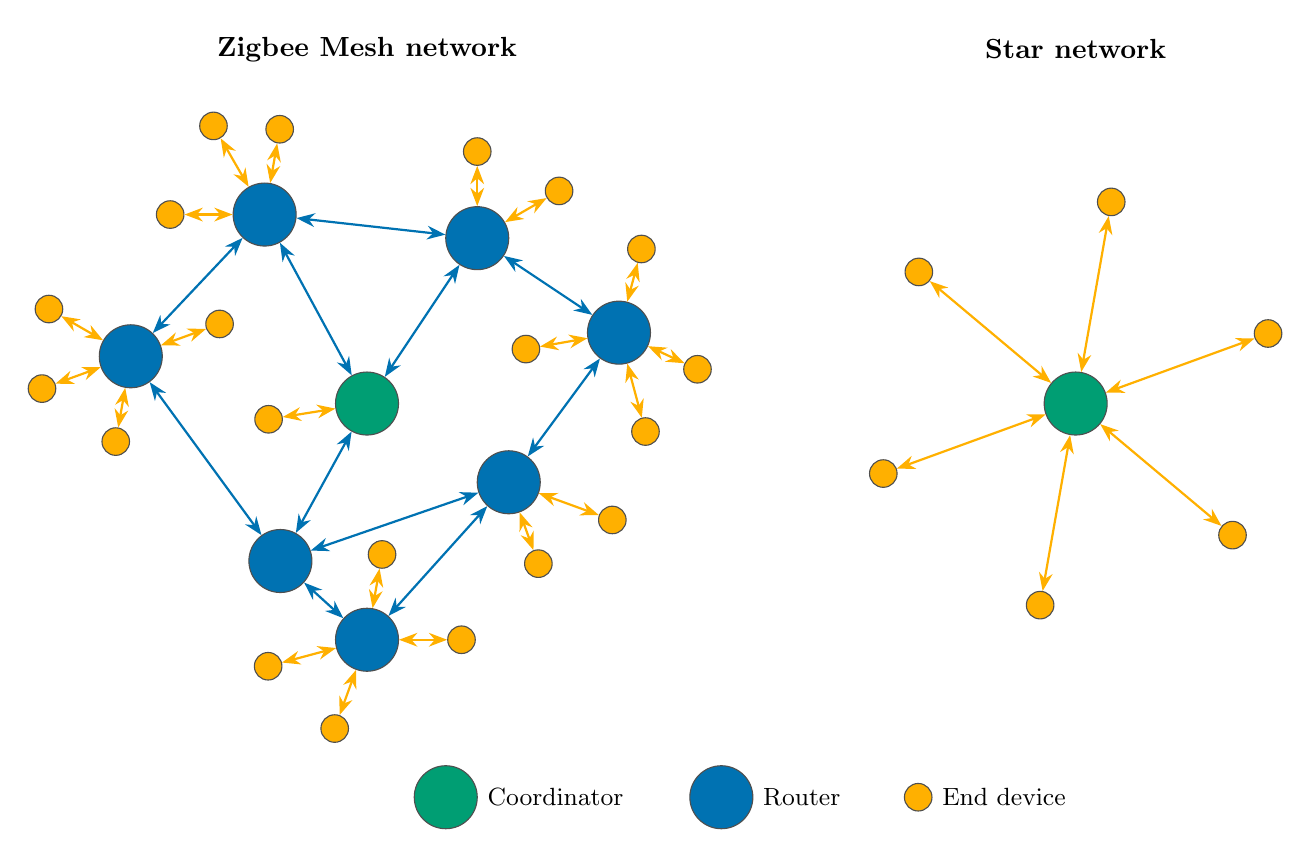
\begin{tikzpicture}[font=\small]

\definecolor{IBM1}{HTML}{648fff}
\definecolor{IBM2}{HTML}{785ef0}
\definecolor{IBM3}{HTML}{dc267f}
\definecolor{IBM4}{HTML}{fe6100}
\definecolor{IBM5}{HTML}{ffb000}
\definecolor{IBM6}{HTML}{d55e00}
\definecolor{IBM7}{HTML}{cc79a7}
\definecolor{IBM8}{HTML}{0072b2}
\definecolor{IBM9}{HTML}{f0e442}
\definecolor{IBM10}{HTML}{009e73}

\tikzset{
  coord/.style={circle, fill=IBM10, draw=black!69, minimum size=8mm},
  router/.style={circle, fill=IBM8, draw=black!69, minimum size=8mm},
  enddev/.style={circle, fill=IBM5, draw=black!69, minimum size=3.5mm},
  link/.style={<->, >=Stealth, thick, IBM5},
  link2/.style={<->, >=Stealth, thick, IBM8}
}

%mesh
\node[font=\bfseries] at (0,4.5) {Zigbee Mesh network};
\node[coord] (mc) at (0,0) {};
\node[router] (r1) at (-3.0,0.6) {};
\node[router] (r2) at (-1.3,2.4) {};
\node[router] (r3) at (1.4,2.1) {};
\node[router] (r4) at (3.2,0.9) {};
\node[router] (r5) at (1.8,-1) {};
\node[router] (r6) at (-1.1,-2.0) {};
\node[router] (r7) at (0,-3) {};

\draw[link2] (mc) -- (r2);
\draw[link2] (mc) -- (r3);
\draw[link2] (mc) -- (r6);
\draw[link2] (r1) -- (r2);
\draw[link2] (r2) -- (r3);
\draw[link2] (r3) -- (r4);
\draw[link2] (r4) -- (r5);
\draw[link2] (r5) -- (r6);
\draw[link2] (r1) -- (r6);
\draw[link2] (r6) -- (r7);
\draw[link2] (r7) -- (r5);

\path (r1) ++(20:1.2) node[enddev] (r1e1) {};
\path (r1) ++(150:1.2) node[enddev] (r1e2) {};
\path (r1) ++(200:1.2) node[enddev] (r1e3) {};
\path (r1) ++(260:1.1) node[enddev] (r1e4) {};
\draw[link] (r1) -- (r1e1);
\draw[link] (r1) -- (r1e2);
\draw[link] (r1) -- (r1e3);
\draw[link] (r1) -- (r1e4);

\path (r2) ++(80:1.1) node[enddev] (r2e1) {};
\path (r2) ++(120:1.3) node[enddev] (r2e2) {};
\path (r2) ++(180:1.2) node[enddev] (r2e3) {};
\draw[link] (r2) -- (r2e1);
\draw[link] (r2) -- (r2e2);
\draw[link] (r2) -- (r2e3);

\path (r3) ++(30:1.2) node[enddev] (r3e1) {};
\path (r3) ++(90:1.1) node[enddev] (r3e2) {};
\draw[link] (r3) -- (r3e1);
\draw[link] (r3) -- (r3e2);

\path (r4) ++(75:1.1) node[enddev] (r4e1) {};
\path (r4) ++(190:1.2) node[enddev] (r4e2) {};
\path (r4) ++(285:1.3) node[enddev] (r4e3) {};
\path (r4) ++(335:1.1) node[enddev] (r4e4) {};
\draw[link] (r4) -- (r4e1);
\draw[link] (r4) -- (r4e2);
\draw[link] (r4) -- (r4e3);
\draw[link] (r4) -- (r4e4);

\path (r5) ++(290:1.1) node[enddev] (r5e1) {};
\path (r5) ++(340:1.4) node[enddev] (r5e2) {};
\draw[link] (r5) -- (r5e1);
\draw[link] (r5) -- (r5e2);

\path (r7) ++(0:1.2) node[enddev] (r7e1) {};
\path (r7) ++(80:1.1) node[enddev] (r7e2) {};
\path (r7) ++(195:1.3) node[enddev] (r7e3) {};
\path (r7) ++(250:1.2) node[enddev] (r7e4) {};
\draw[link] (r7) -- (r7e1);
\draw[link] (r7) -- (r7e2);
\draw[link] (r7) -- (r7e3);
\draw[link] (r7) -- (r7e4);

\node[enddev] (ex) at (-1.25,-0.2) {};
\draw[link] (ex) -- (mc);

%star
\begin{scope}[xshift=9cm]
\node[font=\bfseries] at (0,4.5) {Star network};
\node[coord] (sc) at (0,0) {};
\foreach \ang in {20,80,140,200,260,320} {
  \path (sc) ++(\ang:2.6) node[enddev] (s\ang) {};
  \draw[link] (sc) -- (s\ang);
}
\end{scope}

\node[coord, label=right:Coordinator] at (1,-5) {};
\node[router, label=right:Router] at (4.5,-5) {};
\node[enddev, label=right:End device] at (7,-5) {};
\end{tikzpicture}
\end{document}